\section{The growth function}

\mode<presentation>{
\begin{frame} 
    \begin{center} \huge
        \secname
    \end{center}
    
    \svspace{7mm}
    
    \begin{center}
		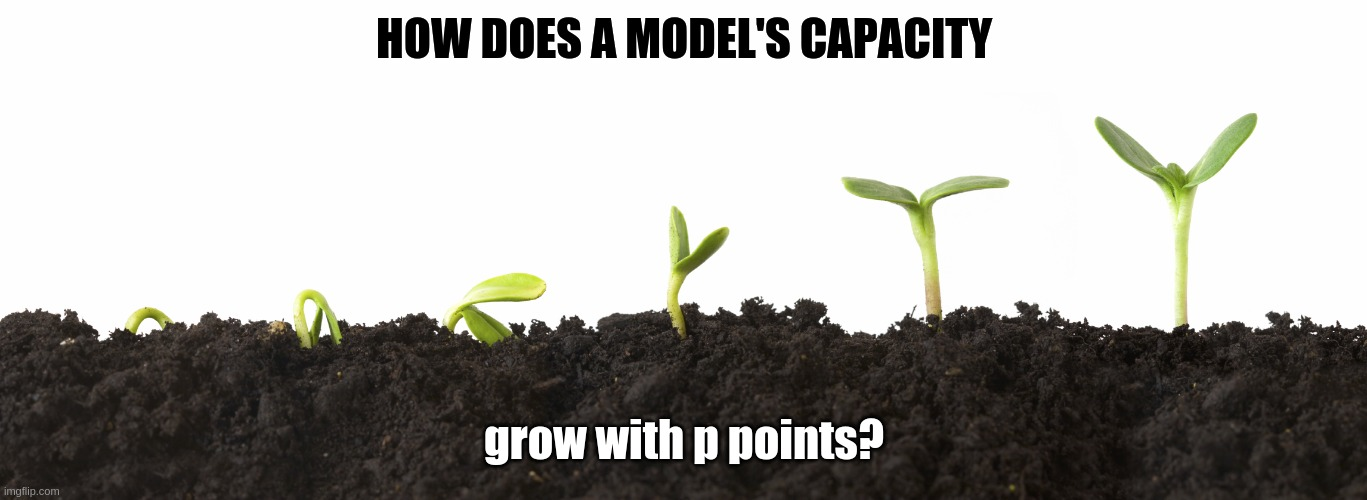
\includegraphics[width=0.6\textwidth]{img/meme_growth}
    \end{center}
\end{frame}
}

\begin{frame}\frametitle{\secname~- What is it?}

The growth function is the measure of \emph{sample} complexity for a model class.\\[5mm]

It measures the complexity of the functions that can be fitted using a model from that model class (e.g. connectionist neuron).\\[5mm]

\emph{sample} complexity: \emph{how much can I do with $p$ points in $N$ dimensions?}\\[10mm]

It is closely related to the \emph{VC dimension}.

\end{frame}

\subsection{Defining the growth function}

\mode<presentation>{
\begin{frame} \frametitle{The growth function $G_{(p)}^\Lambda$}
	\begin{itemize}
		\item \textbf{data representation:} 
			$\vec{x} \in \mathbb{R}^N, \quad y_T \in \{-1,+1\}$ 
		\vspace{5mm}
		\item \textbf{model class:} 
			set $\Lambda$ of functions $y_{(\vec{x}; \vec{w})} \in \{-1,+1\}$
			
		\vspace{5mm}
		\item \textbf{binary label vector:} $\vec y_{(\vec{w})} = \Big( 
			y_{(\vec{x}^{(1)}, \vec{w})}, 
			y_{(\vec{x}^{(2)}, \vec{w})}, \ldots, 
			y_{(\vec{x}^{(p)}, \vec{w})} \Big)$
			\begin{itemize}	
				\item different classifiers can induce the 
					same label vector on the training set 
			\end{itemize}
			
		\vspace{5mm}
		\item \textbf{number of different vectors} $\vec y_{(\vec{w})}$ 
			induced by all $\vec w \in \Lambda$:
			\vspace{-2mm}
			\begin{equation}
				\tag{depends on $\Lambda$ and the sample}
				N_{(\vec{x}^{(1)}, \ldots, \vec{x}^{(p)})}^\Lambda 
				\;\;\leq 2^p 
			\end{equation}
	\end{itemize}
\end{frame}
}


\begin{frame} \frametitle{The growth function $G_{(p)}^\Lambda$}
	\begin{itemize}
		\item<1-> \textbf{data representation:} 
			$\vec{x} \in \mathbb{R}^N, \quad y_T \in \{-1,+1\}$ 
		\vspace{5mm}
		\item<1-> \textbf{model class:} 
			set $\Lambda$ of functions $y_{(\vec{x}; \vec{w})} \in \{-1,+1\}$
			
			Think of $\Lambda$ as a set of classifiers.
			The classifiers in this set come from the same model class (e.g. connectionist neurons with weights $\vec w$).
			Each classifier describes a different hyperplane (different $\vec w$) to separate the two classes in the data.
			
		\vspace{3mm}
		\item<2-> {\textbf{binary label vector}:} $\vec y_{(\vec{w})} = \Big( 
			y_{(\vec{x}^{(1)}, \vec{w})}, 
			y_{(\vec{x}^{(2)}, \vec{w})}, \ldots, 
			y_{(\vec{x}^{(p)}, \vec{w})} \Big)$
			\begin{itemize}	
				\item different classifiers can induce the 
					same label vector on the training set\notesonly{ (cf. \figref{fig:dichotomy_redundant})}
					
				%\begin{center}
					%\includegraphics<2>[width=0.25\textwidth]{img/dichotomy_redundant}
					%\notesonly{
					%\captionof{figure}{Different weight vectors that produce identical labelng of the points.}
					%}
					%\label{fig:dichotomy_redundant}
				%\end{center}
			\end{itemize}
			
			Each classifier in $\Lambda$ describes a different hyperplane.
            \mode<article>{
			Looking at the predictions each one produces for the $p$ points will produce some label vector $\vec y_{(\vec{w})}$ with $p$ elements. A prediction for every point.
			}
		\vspace{5mm}
		\item<3> \textbf{number} of different vectors $\vec y_{(\vec{w})}$ 
			induced by all $\vec w \in \Lambda$:
			\vspace{-2mm}
			\begin{equation}
				\tag{depends on $\Lambda$ and the sample}
				N_{(\vec{x}^{(1)}, \ldots, \vec{x}^{(p)})}^\Lambda 
				\;\;\leq 2^p 
			\end{equation}
	\end{itemize}
\end{frame}

\begin{frame}\frametitle{The growth function $G_{(p)}^\Lambda$ and $N^{\Lambda}$}
		Two hyperplanes can be different but still yield the same predictions.
		Example:\\
		\begin{figure}[h]
			\centering
			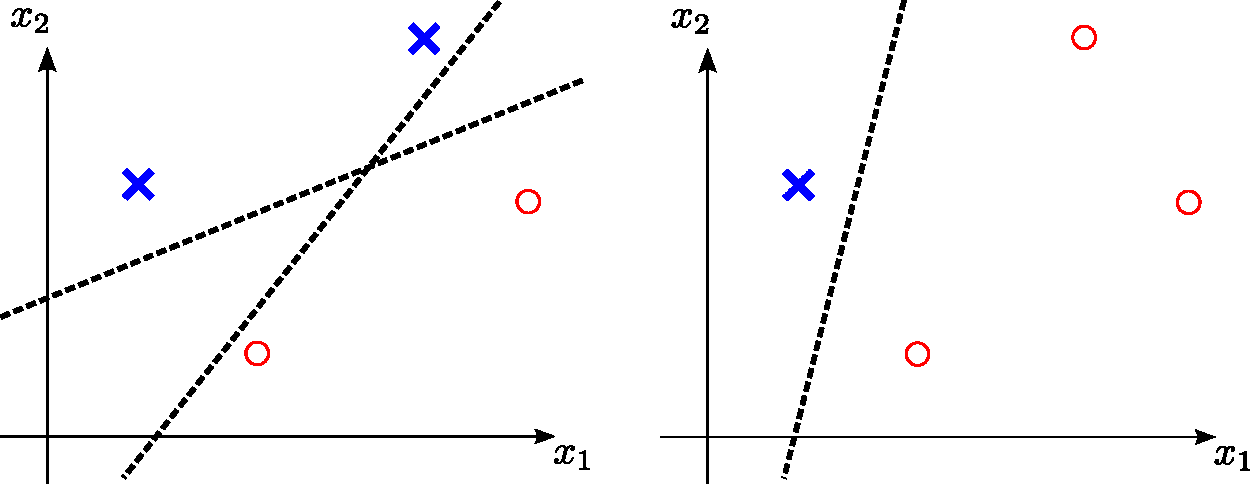
\includegraphics[width=0.6\textwidth]{img/uniquepredictions}
            \mode<article>{
			\caption{Different hyperplanes can lead to different but also to identical labeling of points}
            }
		\end{figure}
		\mode<article>{
		We are interested in the set of unique labeling vectors, more importantly, the size of this set. It tells us how many labeling configuration can be fitted by a model from the model class.
		The number of unique labeling vectors is 
		$N_{(\vec{x}^{(1)}, \ldots, \vec{x}^{(p)})}^\Lambda$
		
		Given that the total number of possible labeling configuration is $2^p$
		and that we cannot guarantee that the models from $\Lambda$ can be fitted to all of them, it follows:
		}
        \begin{equation}
            N_{(\vec{x}^{(1)}, \ldots, \vec{x}^{(p)})}^\Lambda
            \;\;\leq 2^p 
        \end{equation}
\end{frame}

\begin{frame}\frametitle{Defining the growth function $G_{(p)}^\Lambda$}

	\mode<article>{	
		There are various reasons for $N^\Lambda$ to fall below $2^p$. Maybe we didn't sample enough classifiers from $\Lambda$. To eliminate the effects of this ``sampling'' we look for the maximum value \emph{that can be obtained} (supremum) for $N^\Lambda$ and by looking at how this value behaves as a function of $p$ we arrive at the growth function:
		}
		
	%\begin{equation} 
			%G_{(p)}^\Lambda = \ln \underbrace{ \bigg( 
				%\sup_{\vec{x}^{(1)}, \ldots \vec{x}^{(p)}}
				%N_{(\vec{x}^{(1)}, \ldots, \vec{x}^{(p)})}^\Lambda \bigg) }_{
					%\text{worst case}}
	%\end{equation}
	\svspace{-3mm}
	\begin{equation}
	G_{(p)}^\Lambda = \ln \bigg( 
				\sup_{\vec{x}^{(1)}, \ldots \vec{x}^{(p)}}
				N_{(\vec{x}^{(1)}, \ldots, \vec{x}^{(p)})}^\Lambda \bigg) = \ln 2^p = p \ln 2
				\label{eq:growthln2}
	\end{equation}
	
    \notesonly{
	Before we proceed, we turn back to the convergence of ERM, specifically \eqref{eq:absdeltaconvergence0}:
    }
	\mode<presentation>{
    Recall:
    \svspace{-3mm}
				\begin{equation*}
				\lim_{p \to \infty} P\bigg\{ 
					{
						\Big|R_{[\vec w_p]} - R_{[\vec w_0]}\Big| 
					}
				\geq \eta \bigg\}\;\;=\;\; 0 \,, \quad \forall \eta > 0
			\end{equation*}
	}
	
	This convergence is equivalent to\footnote{\notesonly{We don't dig into how they are equivalent. }If interested, see Ch. 5.5 \citep{scholkopf2001learning} for a description of the approach and \citep{vapnik1999overview} for the detailed derivation.
	}:
	\begin{equation}
	\lim_{p \to \infty} G_{(p)}^\Lambda / p \eqexcl 0
	\end{equation}
	\mode<article>{
	In the case of $G_{(p)}^\Lambda = p \ln 2$ as per our definition of the growth function in \eqref{eq:growthln2}:
	}
	\begin{equation}
	\lim_{p \to \infty} \left( p \ln 2 \right ) / p = \ln 2 \ne 0
	\end{equation}
	
	\notesonly{
	There is no convergence to zero, regardless of $p$. According to Vapnik, this means that} the classifier's predictions become ambiguous and will likely fail to generalize.

\end{frame}

\begin{frame}{Complete ambiguity}
    The growth function does not tell us how many points we need to separate the two classes but how many points we need to exclude completely ambiguous predictions.\\
    
\end{frame}

\begin{frame}{Example with complete ambiguity}
    \notesonly{Example with complete ambiguity:\\}
    \mode<presentation>{
    
    Linear neuron, 2 points in 2D. We do not have access to the hyperplane $\vec w$. We only have access to the predictions made by the neuron:\\
    %\textbf{see blackboard\ldots}
    }
    
	\begin{center}
\slidesonly{
		\includegraphics<2>[width=0.3\textwidth]{img/dichotomy_ambiguous}
		\includegraphics<3>[width=0.3\textwidth]{img/dichotomy_ambiguous_new_point}
		}
		\includegraphics<4>[width=0.3\textwidth]{img/dichotomy_ambiguous_decision_boundaries}
		\notesonly{
		\captionof{figure}{Ambiguous regions. No complete ambiguity for this particular case yet, but still possible.}
		}
	\end{center}
\slidesonly{
\only<4>{
	\begin{center}
		Ambiguity not \textbf{yet} complete.
	\end{center}
		}
		}

\only<5>{
\begin{center}
\begin{minipage}{0.45\textwidth}
\begin{center}
	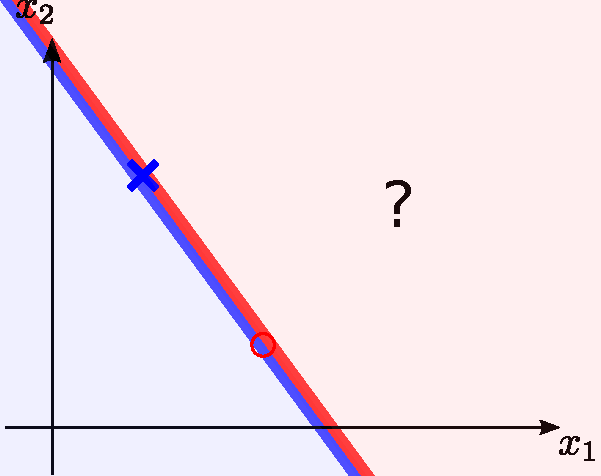
\includegraphics[width=0.7\textwidth]{img/dichotomy_ambiguous_decision_boundaries_2}
\end{center}
\end{minipage}
\begin{minipage}{0.45\textwidth}
\begin{center}
	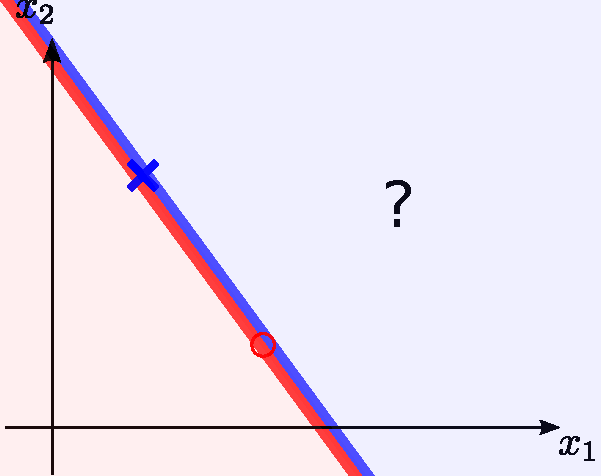
\includegraphics[width=0.7\textwidth]{img/dichotomy_ambiguous_decision_boundaries_3}
\end{center}
\end{minipage}
	\notesonly{
	\captionof{figure}{Complete ambiguity over the label of a third point, when we only have the predictions of two points in 2D by a linear neuron.}
	}
\end{center}
}
    
    \mode<article>{Any linear neuron can find a hyperplane to separate two specific points in 2-D space. It does not tell us anything about the neuron's ability to separate an additional 3rd test point in that same space. Therefore $p = 2$ is still ambiguous for the linear neuron.}
    
\end{frame}

\begin{frame}{Example with \textbf{non}complete ambiguity}
    \notesonly{An example with \textbf{no complete} ambiguity:\\}
    \mode<presentation>{
    
    Linear neuron, 3 points in 2D:\\
    %\textbf{see blackboard\ldots}
    }
    
	\begin{center}
\slidesonly{
		\includegraphics<1>[width=0.3\textwidth]{img/dichotomy_nonambiguous_new_point}
		}
		\includegraphics<2>[width=0.3\textwidth]{img/dichotomy_nonambiguous_decision_boundaries}
		\notesonly{
		\captionof{figure}{No complete ambiguity over the label of the third point in 2D.}
		}
	\end{center}
\end{frame}

\mode<article>{
\begin{frame}
However, for $p > \dvc$ the growth function behaves differently, namely
	\begin{equation}
		G^{\Lambda}_{(p)} \le \dvc \cdot \Big(1+ ln \frac{p}{\dvc}\Big)
	\end{equation}
	
	In this case  $\lim_{p \to \infty} G_{(p)}^\Lambda$ converges to zero, and there is no more complete ambiguity. There is at least one region in feature space where all different classifiers from $\Lambda$ will agree on what class to assign to points in that region. There may still exist regions for which predictions will be ambiguous but the complete ambiguity is gone. The more points we add, the less likely a model will find a solution, but if it does, they will no longer be ambiguous.

%Maybe this provokes the question: Why is the plot even useful? If I change my model to something with a lower d_VC, all I'm doing is that I allow the linear part of G to stop and switch to the curvy part earlier. A lower d_VC means that the curvy part happens for less p where the p ln 2 is also lower. The range of ambiguous predictions becomes lower and I'm able to generalize with fewer training samples.
\end{frame}
}

\begin{frame}
	\begin{itemize}
		\item bound on growth function (Vapnik, 1998)
			\begin{equation}
				G_{(p)}^\Lambda
				\left \{ \begin{array}{ll}
					= p \ln 2 
					& \text{for } p \leq \dvc \\
					\leq \dvc \cdot \Big( 1 + \ln \frac{p}{\dvc} \Big) 
					& \text{for } p > \dvc
				\end{array} \right.
			\label{eq:growthpiecewise}
			\end{equation}

		\item Vapnik-Chernovenkis dimension $\dvc$: \\
			capacity measure of the model class
		%\itR the growth function is independent of a specific sample
		%\itR the growth function is bounded by a term logarithmic in $p$
		%\itR the growth rate depends on the model's VC-dimension $\dvc$ 
	\end{itemize}
\end{frame}

% -----------------------------------------------------------------------------
\begin{frame}\frametitle{The growth function $G_{(p)}^\Lambda$}
	\begin{center}
		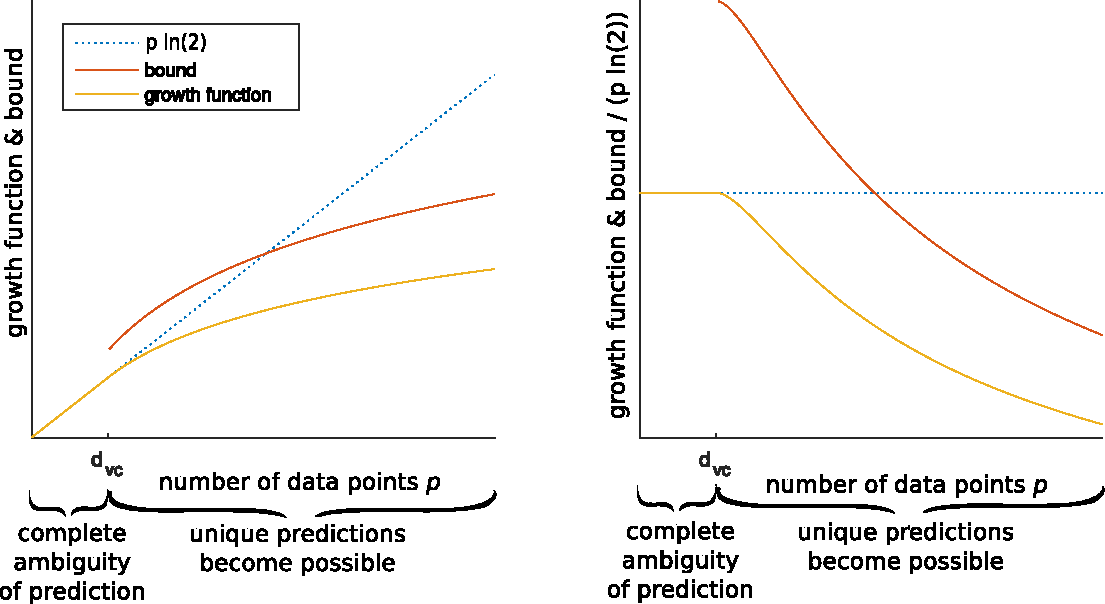
\includegraphics[height=5.7cm]{img/growth_function_clean}
	\end{center}
	\vspace{-2mm}
	$\dvc$: capacity measure of the model class\\
	small $\dvc$: small sample size sufficient for learning\\
	large $\dvc$: large sample size required

		%\item growth function defines VC-dimension $\dvc$
		%\item higher capacity $\rightarrow$ more different labelings
\end{frame}



\subsection{Revisit convergence of ERM}
\mode<article>{
\begin{frame}\frametitle{\subsecname}\label{sec:convergence_erm_revisit}
			
			Convergence of Empirical risk minimization is guaranteed:
			
			For a model class with \emph{finite} $\dvc$\notesonly{, the empirical training error will converge to the generalization error
			with more data. That is:}
			\begin{equation}
				\lim_{p \to \infty}
						E^T_{[\vec w]} = E^G_{[\vec w]}
			\end{equation}
			
			The requirement is that $\dvc$ is \emph{finite}.
			
			\mode<article>{The training error converges to the generalization error.
			}
			In terms of risk, this would be:
			
			\begin{equation}
				\lim_{p \to \infty} 
					R_{\text{emp}[\vec w]} = R_{[\vec w]}
			\end{equation}
			
			\begin{equation}
				\lim_{p \to \infty} P\bigg\{ 
					{
						\Big|R_{(\vec w_p)} - R_{(\vec w_0)}\Big| 
					}
				\geq \eta \bigg\}\;\;=\;\; 0 \,, \quad \forall \eta > 0
				\label{eq:risktozero}
			\end{equation}
			
			\textbf{But} Our dataset is never going to be infinitely large. Therefore, a more realistic formulation would be that ERM converges to some small $\epsilon$.\\
			We therefore reiterate \eqref{eq:convergenceeps}:
			
			\begin{equation}
				\lim_{p \to \infty} P\bigg\{ 
					{
						\Big|R_{(\vec w_p)} - R_{(\vec w_0)}\Big| 
					}
				\geq \eta \bigg\}\;\;<\;\; \epsilon \,, \quad \forall \eta > 0
				\label{eq:risktozero}
			\end{equation}
			
			The takeaway from the growth function and the bounds is that it defines the value of $\eta$ in \eqref{eq:convergenceeps} that can be targeted when training a specific model with a finite set of $p$ points.
			
			
\end{frame}
}

%TODO
%We replace  
%η
  %by this juggernaut term. We don't ask you to reproduce it. The important thing is to understand what happens when you select a larger value for p. The bound becomes tighter. This should not come as a surprise. In #30 we had the case of p approaching infinity which allowed us to bound everything by some constant  
%η
 %. Slide #31 expands this constant into terms that are a function of p. The bound has to be sensitive to p. #31 does not add new information but only rearranges the terms to being back  
%η
  %and express the confidence in terms of the size of the data set instead of  
%ϵ
 %.
 


\begin{frame}\frametitle{The solution to learning problem 2} 
	\begin{center}
		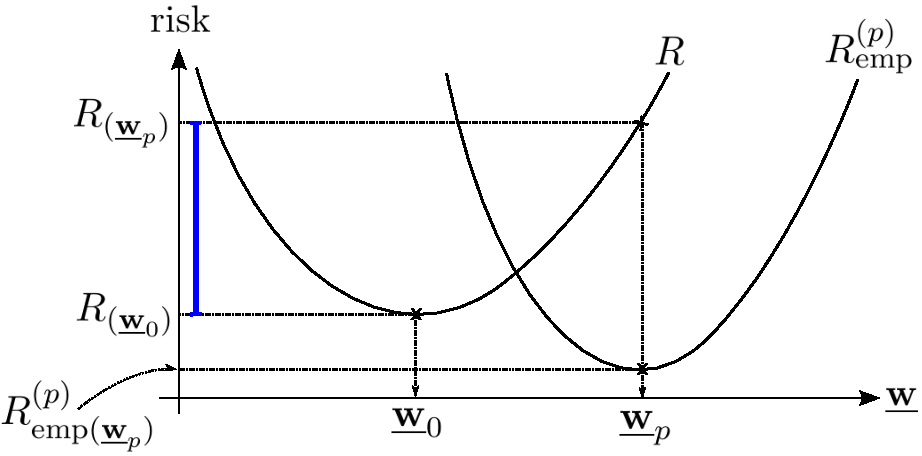
\includegraphics[width=9cm]{img/section2_fig1_question1}
	\end{center}
	\begin{enumerate}\setcounter{enumi}{1}
		\item \textbf{finite samples:} deviation from the optimal model
			\vspace{-2mm}
			\begin{equation}
				P\bigg\{ {%\color{question1} 
				{\color{blue}\Big| R_{(\vec w_p)} - R_{(\vec w_0)} \Big|} }
					> \Big(\smallfrac{G^\Lambda_{(2p)} 
						- \ln \frac{\epsilon}{8}}{p} \Big)^\frac{1}{2}
					+ \Big(-\smallfrac{\ln \frac{\epsilon}{2}}{2p} 
						\Big)^\frac{1}{2} + \smallfrac{1}{p}
				\bigg\} < \epsilon
					\label{eq:boundgenerlizationdeviation}
			\end{equation}
			\vspace{-4mm}
			\iitem{ finite $\dvc$: increased sample size $p$ 
				$\Rightarrow$ reduction of the bound}
	\end{enumerate}
\end{frame}

\mode<presentation>{
\begin{frame}\frametitle{Re-thinking $\eta$: bounded by the growth function}
\begin{center}
	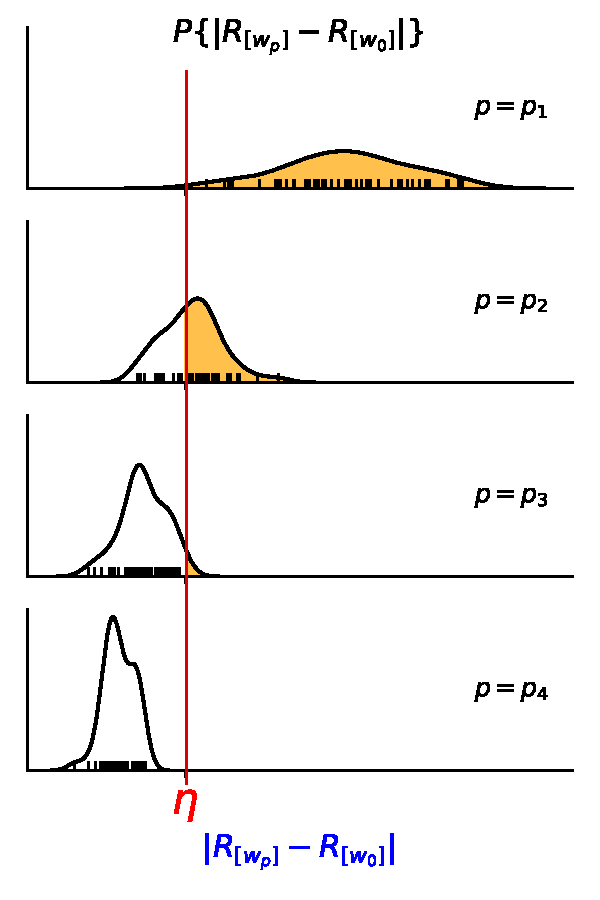
\includegraphics[height=6cm]{img/PdeltaReta}
\end{center}
			%\begin{equation}
				%\lim_{p \to \infty} P\bigg\{ 
					%{
						%\Big|R_{(\vec w_p)} - R_{(\vec w_0)}\Big| 
					%}
				%\geq \eta \bigg\}\;\;<\;\; \epsilon \,, \quad \forall \eta > 0
				%\label{eq:risktozero}
			%\end{equation}
						\begin{equation}
				P\bigg\{ {%\color{question1} 
				{\color{blue}\Big| R_{(\vec w_p)} - R_{(\vec w_0)} \Big|} }
					> \Big(\smallfrac{G^\Lambda_{(2p)} 
						- \ln \frac{\epsilon}{8}}{p} \Big)^\frac{1}{2}
					+ \Big(-\smallfrac{\ln \frac{\epsilon}{2}}{2p} 
						\Big)^\frac{1}{2} + \smallfrac{1}{p}
				\bigg\} < \epsilon
					\label{eq:boundgenerlizationdeviation}
			\end{equation}
\end{frame}
}

\mode<article>{
Recall that we were using \figref{fig:PdeltaReta} to see how the probability of scoring non-zero training error vanishes with more data points.
More data is good and the distribution of errors shifts to the left of $\eta$. While doing so, we were treating $\eta$ as a constant.

After learning about the growth function, we discover that $\eta$ is not necessarily an arbitrary constant but a value that is tied to the growth function of the model class \underline{and} the number of training points $p$\footnote{If interested, the supplementary material derives the relationship between $\eta$, the growth function and $p$}. Knowing that this relationship exists we learn that the vertical line we drew at $\eta$ is capable of shifting as a result of varying $p$ and the growth function.

Increasing $p$ not only causes the distribution to shift to the left but also
causes $\eta$ to shift to the left. Both will not necessarily shift at the same rate but
it just means that increasing $p$ no longer guarantees probability of
zero. The bound gets \textit{lower} with larger $p$. Why should we not be surprised by
this? One word: underfitting. Increasing $p$ and not getting rid of error is
indicative of a bias in our model class. It will not benefit from throwing
more data at it.

A larger growth function shifts the $\eta$ line to the right. The
distribution shifts to the right, so both are moving away from each other. The
probability of error vanishes and we get zero error on the training set. It's important to remember that the zero
error will only occur on the training set. Forgetting about it will make us
think choosing a larger growth function will always make us generalize
better and this is simply not the case. This is why we need to bound the probability by the
generalization capabilities of the model class which leads us to the following formulation:
}

\begin{frame}\frametitle{The solution to learning problem 3} 
	\begin{center}
		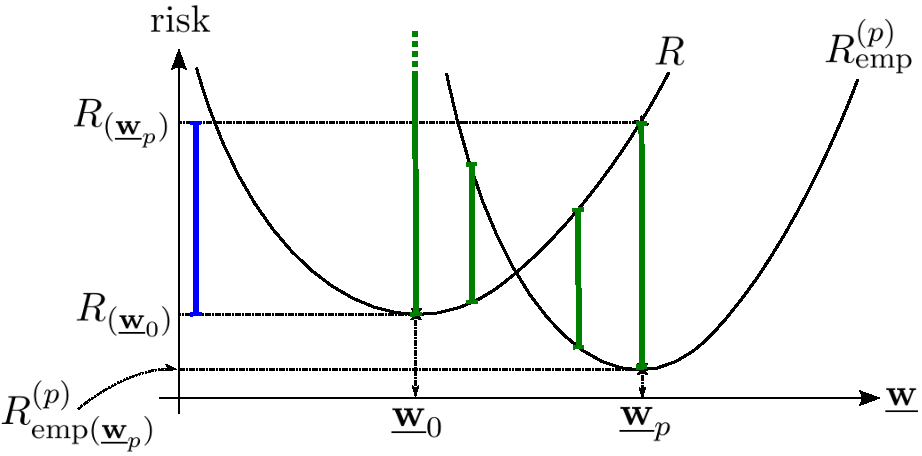
\includegraphics[width=9cm]{img/section2_fig1_question2_lessw}
	\end{center}
	\begin{enumerate}\setcounter{enumi}{2}
		\item \textbf{finite samples:} bound on the generalization error
			\vspace{-2mm}
			\begin{equation}
				P\bigg\{ \sup\limits_{\vec w \in \Lambda}
					{%\color{question2} 
						\Big|R_{(\vec w)} - R^{(p)}_{\text{emp}(\vec w)}\Big| 
					} > \eta
				\bigg\} < 4 \exp\Big( G^\Lambda_{(2p)} 
					- p \big( \eta - \smallfrac{1}{p} \big)^2 \Big)
					\label{eq:boundgenerlization}
			\end{equation}
			\vspace{-4mm}
			\iitem{ bound non-trivial only if $G^\Lambda_{(2p)}$ 
				is sub-linear in $p$}
	\end{enumerate}
\end{frame}
